\chapter{Arhitektura i dizajn sustava}

    \hfill\break
    Arhitektura se može podijeliti na tri podsustava: 
    \begin{itemize}
		\item \textbf{Web poslužitelj} 
		\item \textbf{Web aplikacija } 
		\item \textbf{Baza podataka } 
	\end{itemize}
	\hfill\break	
	
	\textbf{Web preglednik} je aplikacija za pristup World Wide Web-u. Kada korisnik želi otvoriti web stranicu, web preglednik šalje HTTP protokol preko kojega zahtjeva sadržaj stranice. Nakon što dobije sadržaj stranice web preglednik ga prevodi i prikazuje korisniku kao jasno i razumljivo grafičko sučelje. 
	\newline \newline
	
	\textbf{Web poslužitelj} je računalo na kojem se izvodi aplikacija.Njegova glavna zadaća je prihvaćanje zahtjeva putem HTTP protokola. Poslužitelj šalje zahtjeve web aplikaciji na obradu i korisniku vraća odgovor.
	\newline \newline
	
	\textbf{Web aplikacija} je zaslužna za obradu korisničkih zahtjeva. Ima pristup bazi podataka. Odgovore šalje u obliku HTML dokumenta web poslužitelju koji ih prosljeđuje korisniku. Arhitektura aplikacije se može podijeliti na front-end i back-end. Cijeli sustav se poslužuje pomoću \textbf{digitalOcean-a}
	\newline\newline
	
	Za izradu backend dijela naše aplikacije odabrali smo radni okvir Spring Boot. Programski jezik koji koristimo je Java.\newline Struktura toga dijela aplikacije biti će troslojna:
	\begin{itemize}
		\item \textbf{Controller} je sloj na kojem se nalazi naš REST API
		\item \textbf{Service} sloj upravlja poslovnom logikom naše aplikacije
		\item \textbf{Repository} sloj služi za pristup podatcima u bazi podataka
	\end{itemize}
					    
	\begin{figure}[H]
        \centering
        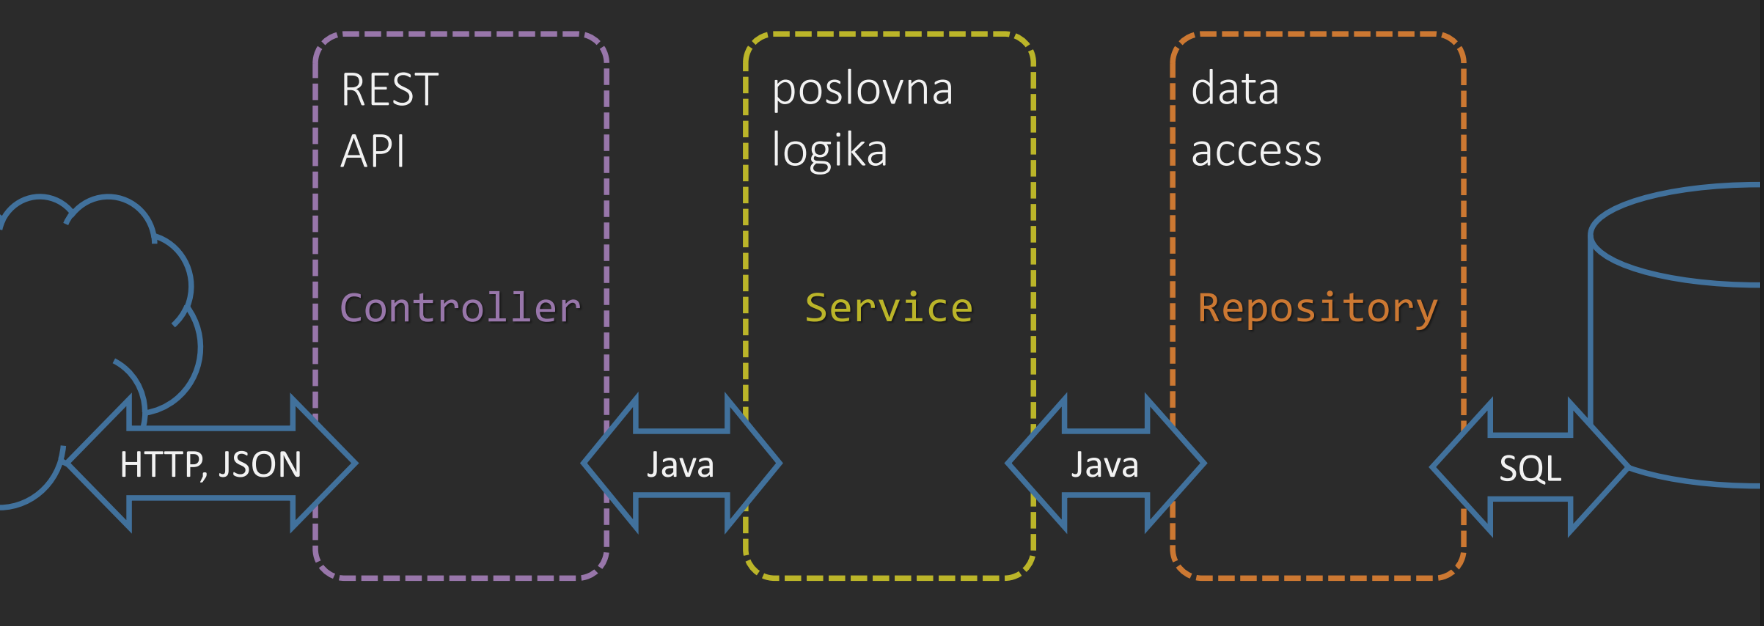
\includegraphics[width=\textwidth]{img/SpringBootflowArchitecture.png}
        \caption{Prikaz troslojne strukture Spring Boot radnog okvira}
    \end{figure}
	\hfill\break
	Za izradu frontend dijela naše aplikacije odabrali smo Javascript library React. Uz React su nam potrebni i alat node.js te upravitelj paketa npm.  

    \section{Baza podataka}
    Analizom zahtjeva utvrđeno je da aplikacija treba podržavati više korisnika koji istodobno mogu pregledavati, uređivati, stvarati i/ili brisati podatke bez da se pojave nekonzistentnosti. Podatci koje je potrbeno spremati, unaprijed su poznati i dobro definirani, a nisu prirodno strukturirani kao graf pa je relacijska baza podataka izabrana kao najbolje rješenje za pohranu podataka.Za bazu podataka smo koristili Postgresql.
    \eject
    
    \subsection{Opis tablica}
        \hfill\break
        Entitet Račun sadrži informacije koje su iste za svakog korisnika i koje korisnik unosi prilikom registracije. Atributi računa su: ID računa koji se dodijeljuje automatski, email, lozinku, opis, vrsta korisnika (osnovni ili vlasnik obrta). Atribut zaključano je postavljen na false, a mijenja se na true ako korisnik više puta pogriješi lozinku. Omogućeno se postavlja na true ako je račun aktivan.
        \hfill\break
	    \begin{tblr}{
                hlines = {},
                colspec={|X[9,l]|X[7, l]|X[15, l]|}, 
                cell{1}{1} = {c = 3}{halign = c}
            }
            {\bf account} (Račun) &    &    \\
            \SetRow{LightGreen} account\textunderscore id & INT & identifikator  \\
            email & VARCHAR(50) & adresa e-pošte \\
            password & VARCHAR(60) & enkriptirana lozinka \\
            bio & VARCHAR(200) & biografija \\
            user\textunderscore role & VARCHAR(10) & razina autorizacije korisnika \\
            locked & BOOLEAN & istina ako korisnik više puta unese pogršnu lozinku \\
            enabled & BOOLEAN & istina ako je račun aktivan 
        \end{tblr}
        \hfill\break
        
        Nakon ispunjavanja registracijske forme korisnik na mail dobiva link kojim potvrđuje račun. Ta potvrda se sprema u tablicu Token za potvrdu računa. Tablica sadrži atribute ID tokena za potvrdu, token za potvrdu, datum kreiranja u kojima se bilježe podatci o tokenu te ID računa potreban da se poveže s računom koji se aktivira.
        \hfill\break
        \begin{tblr}{
                hlines = {},
                colspec={|X[9,l]|X[7, l]|X[15, l]|}, 
                cell{1}{1} = {c = 3}{halign = c}
            }
            {\bf confirmation\textunderscore token } (Token za potvrdu računa) &    &    \\
            \SetRow{LightGreen} confirmation\textunderscore token\textunderscore id & INT & identifikator  \\
            confirmation\textunderscore token & VARCHAR(36) & token za potvrdu računa\\
            created\textunderscore date & DATE & datum kreiranja tokena \\
            \SetRow{LightBlue} account\textunderscore id & INT & iden. računa za koji je vezan token \\
        \end{tblr}
        \hfill\break
        
        Tablica Korisnički račun sadrži atribute vezane uz osnovnog korisnika. Atribut ID računa posuđen je iz tablice račun uz koji se veže. Dodatni atributi su još korisničko ime, ime i prezime.
        \hfill\break
        \begin{tblr}{
                hlines = {},
                colspec={|X[9,l]|X[7, l]|X[15, l]|}, 
                cell{1}{1} = {c = 3}{halign = c}
            }
            {\bf user\textunderscore account} (Korisnički račun) &    &    \\
            \SetRow{LightGreen} account\textunderscore id & INT & posuđeni ključ  \\
            username & VARCHAR(30) & korisiničko ime \\
            first\textunderscore name & VARCHAR(30) & ime \\
            last\textunderscore name & VARCHAR(30) & prezime 
        \end{tblr}
        \hfill\break
        
        Poslovni račun je tablica za drugi tip korisnika. Također od entiteta račun posuđuje atribut ID računa, a uz njega još sadrži ime obrta, OIB, kontakt broj i ID tipa obrta.
        \hfill\break
        \begin{tblr}{
                hlines = {},
                colspec={|X[9,l]|X[7, l]|X[15, l]|}, 
                cell{1}{1} = {c = 3}{halign = c}
            }
            {\bf business\textunderscore account} (Poslovni račun) &    &    \\
            \SetRow{LightGreen} account\textunderscore id & INT & posuđeni ključ  \\
            business\textunderscore name & VARCHAR(30) & ime obrta \\
            oib & CHAR(11) & oib \\
            phone\textunderscore number & VARCHAR(15) & broj telefona \\
            \SetRow{LightBlue} business\textunderscore type\textunderscore id & INT & ključ relacije bussinesType \\
        \end{tblr}
        \hfill\break

        Tablica lista obrta povezana je preko atributa ID tipa obrta s poslovnim računom i u nju se sprema tip obrta.
        \hfill\break
        \begin{tblr}{
                hlines = {},
                colspec={|X[9,l]|X[7, l]|X[15, l]|}, 
                cell{1}{1} = {c = 3}{halign = c}
            }
            {\bf business\textunderscore type} (Vrsta obrta) &    &    \\
            \SetRow{LightGreen} business\textunderscore type\textunderscore id & INT & identifikator  \\
            business\textunderscore type & VARCHAR(30) & vrsta obrta
        \end{tblr}
        \hfill\break

        Tablica Lokacija sadrži atribut ID lokacije koji nam je potreban za povezivanje ostalih entiteta vezanih uz lokaciju. Osim toga sadrđi još atribute za geografsku dužinu i širinu, adresu, ime lokacije i njezin opis, datum i vrijeme kreiranja. Atribut promovirana je postavljen na nulu osim ako se radi o promoviranoj lokaciji (obrt). Atribut "dog friendly" je boolean koji je true ako je lokacija prikladna za pse. U tablici se također sprema i ID računa korisnika koji ju je kreirao te se još postavlja ID tipa lokacije.
        \hfill\break
        \begin{tblr}{
                hlines = {},
                colspec={|X[9,l]|X[7, l]|X[15, l]|}, 
                cell{1}{1} = {c = 3}{halign = c}
            }
            {\bf location} (Lokacija) &    &    \\
            \SetRow{LightGreen} location\textunderscore id & INT & identifikator  \\
            longitude & NUMERIC(8,5) & longituda \\
            latitude & NUMERIC(8,5) & latituda \\
            address & VARCHAR(50) & adresa \\
            location\textunderscore name & VARCHAR(30) & ime lokacije \\
            location\textunderscore description & VARCHAR(200) & opis lokacije \\
            date\textunderscore time\textunderscore created & TIMESTAMP & vrijeme i datum objave lokacije \\
            promoted & INT & nije nula ako je lokacija promovirana\\
            dog\textunderscore friendly & BOOLEAN & je li lokacija prikladna za pse \\
            account\textunderscore id & INT & identifikator korisnika koji je stvorio lokaciju \\
            \SetRow{LightBlue} location\textunderscore type\textunderscore id & INT & identifikator vrste lokacije
        \end{tblr}
        \hfill\break

        Tip lokacije je tablica koja se preko atributa ID tipa lokacije povezuje se prethodnom tablicom, a dodatno još ima atribut tip lokacije u koji se on upisuje.
        \hfill\break
        \begin{tblr}{
                hlines = {},
                colspec={|X[9,l]|X[7, l]|X[15, l]|}, 
                cell{1}{1} = {c = 3}{halign = c}
            }
            {\bf location\textunderscore type} (Tip lokacije) &    &    \\
            \SetRow{LightGreen} location\textunderscore type\textunderscore id & INT & identifikator  \\
            location\textunderscore type & VARCHAR(30) & vrsta lokacije
        \end{tblr}
        \hfill\break

        Posljednja tablica je Ocjena. U nju se spremaju atributi potrebi za prikaz ocjene određene lokacije. Preko atributa ID lokacije se povezuje s lokacijom na koju se odnosi, a ID računa zapisuje tko je postavio tu ocjenu. Ostali atributi su vrijeme i datum kreiranja, broj zvijezdica i poruka uz ocjenu.
        \hfill\break
        \begin{tblr}{
                hlines = {},
                colspec={|X[9,l]|X[7, l]|X[15, l]|}, 
                cell{1}{1} = {c = 3}{halign = c}
            }
            {\bf review} (Ocjena) &    &    \\
            \SetRow{LightGreen} location\textunderscore id & INT & idn. lokacije za koju je napisana ocjena  \\
            \SetRow{LightGreen} account\textunderscore id & VARCHAR(30) & idn. korinika koji je napisao ocjenu \\
            date\textunderscore time\textunderscore created & TIMESTAMP & vrijeme i datum objave ocjene \\
            stars & FLOAT & ocjena lokacije između 1 i 5 \\
            message & VARCHAR(200) & tekst ocjene
        \end{tblr}
				
			
	\subsection{Dijagram baze podataka}
		\begin{figure}[H]
    		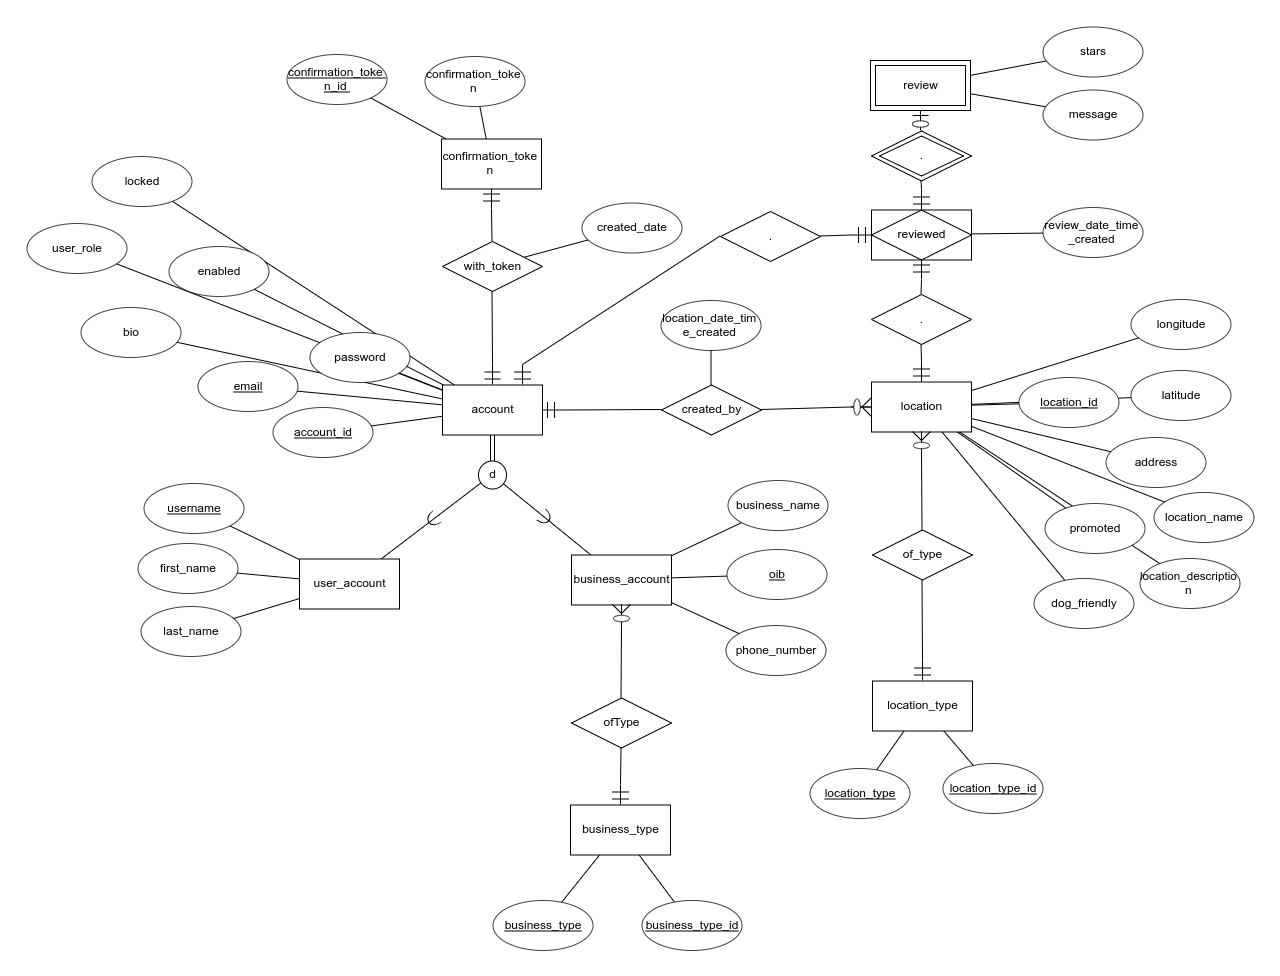
\includegraphics[width=\textwidth]{img/er_dijagram.png}
    		\centering
    		\caption{ER dijagram baze podataka}
    		\label{fig:promjene}
    	\end{figure}

        \begin{figure}[H]
    		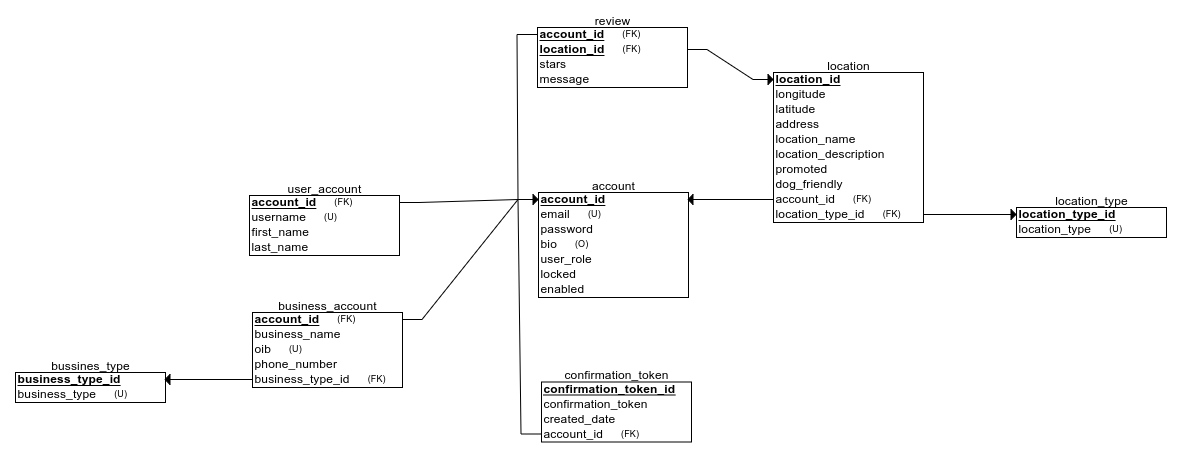
\includegraphics[width=\textwidth]{img/rel_dijagram.png}
    		\centering
    		\caption{Relacijski dijagram baze podataka}
    		\label{fig:promjene}
    	\end{figure}
			
	\eject
        
    
    \section{Dijagram razreda}
        \begin{figure}[H]
        	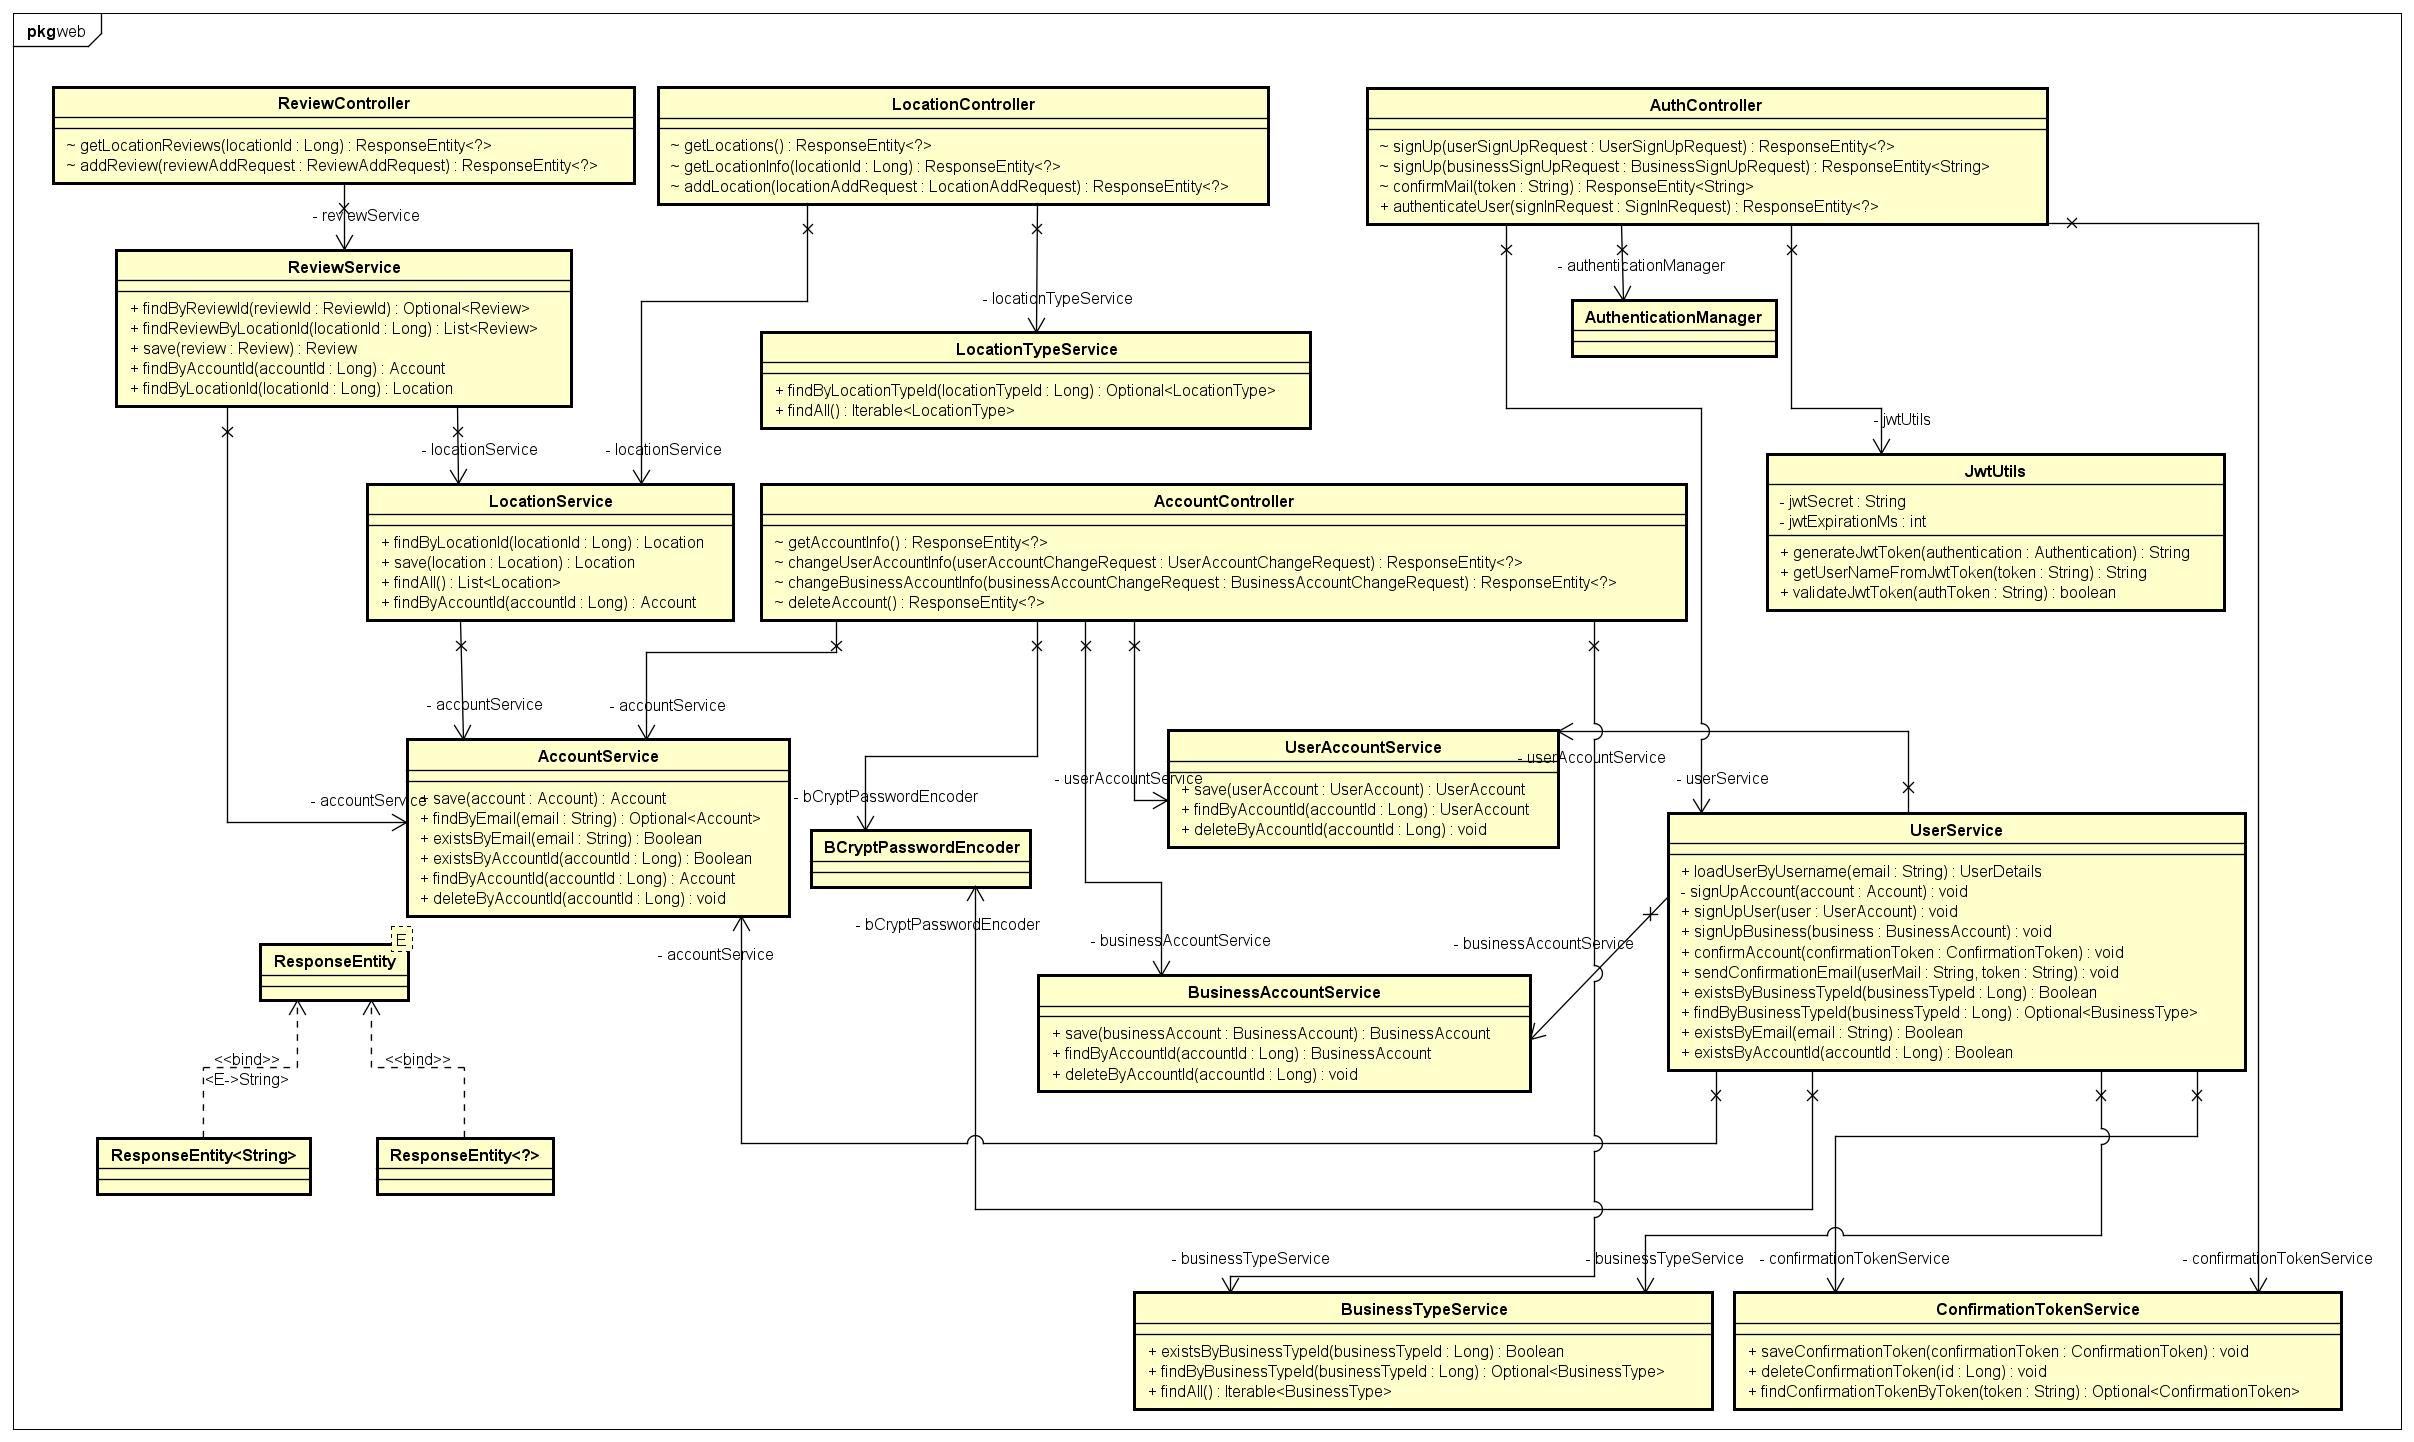
\includegraphics[width=\textwidth]{img/Dijagrami razreda/Controller_Class_Dijagram.jpg}
        	\centering
        	\caption{Controller class}
        	\label{fig:promjene}
        \end{figure}
        \begin{figure}[H]
        	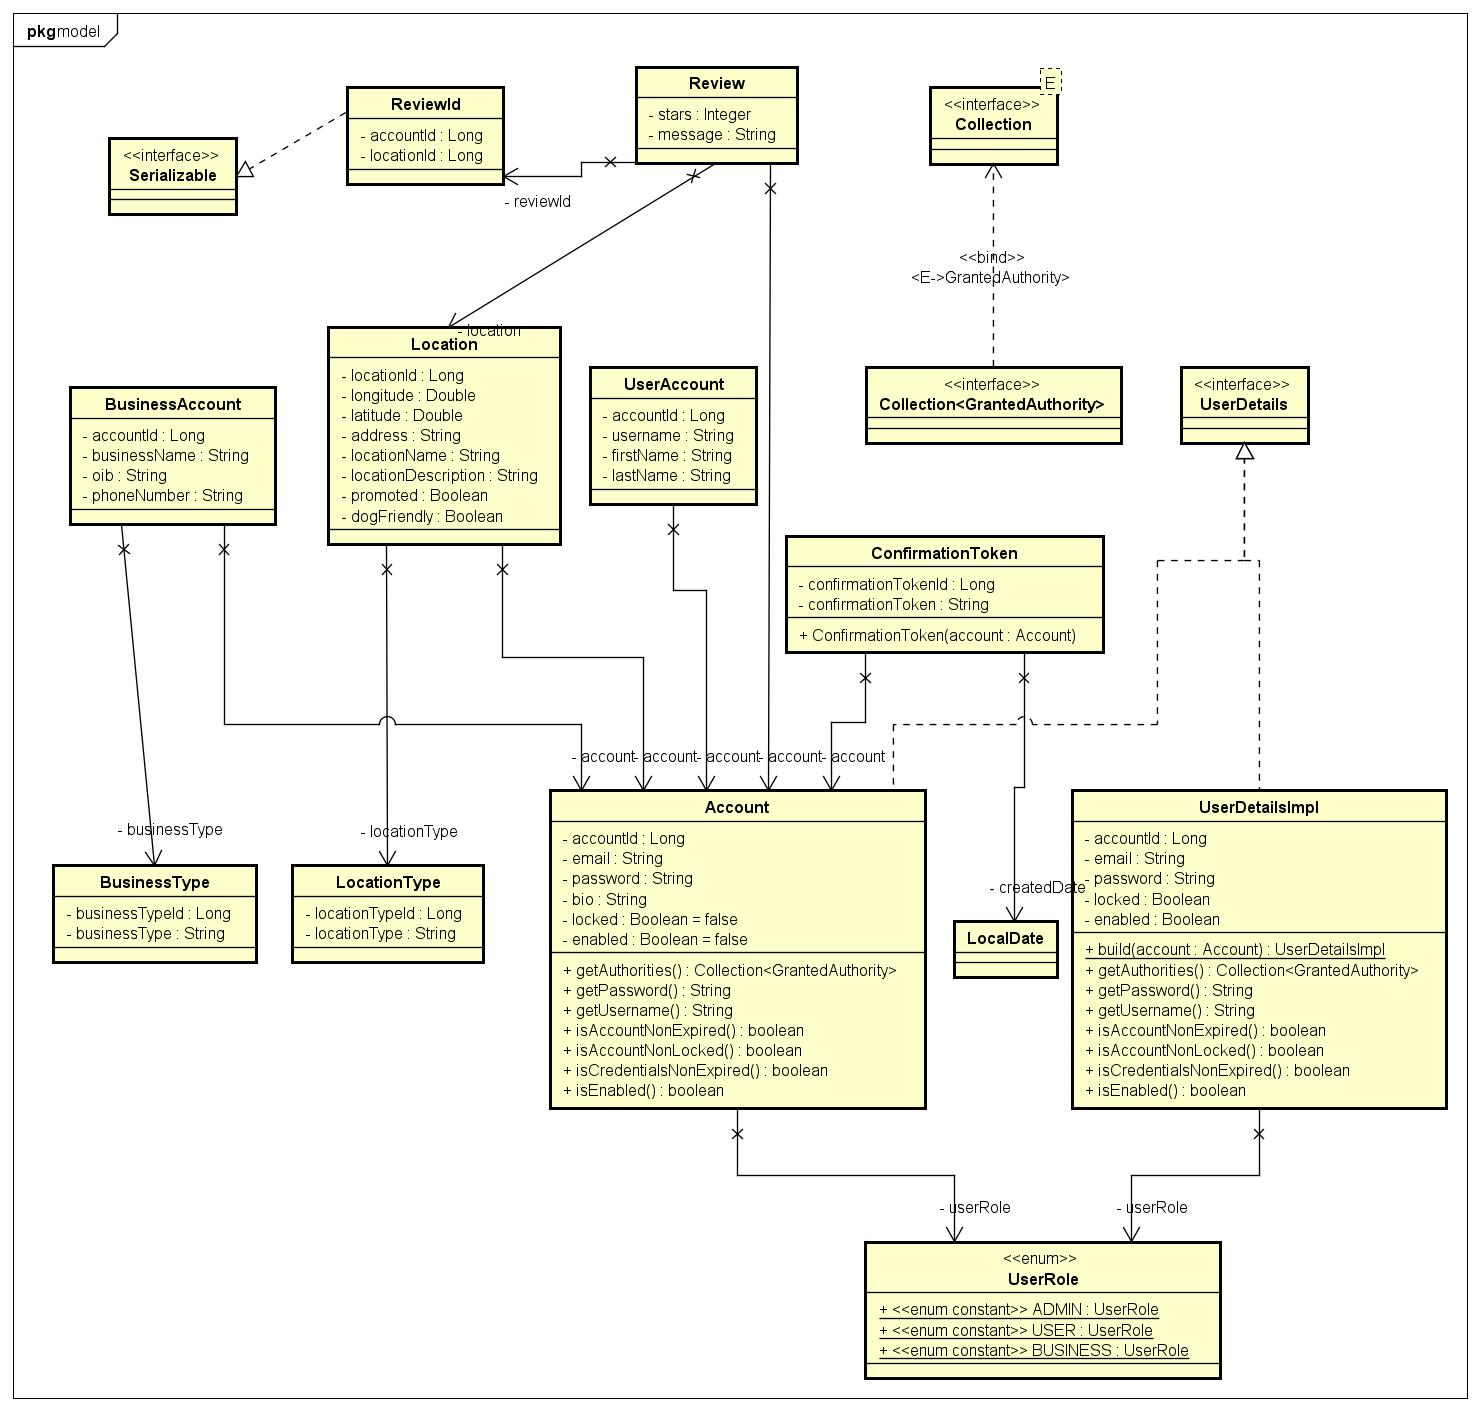
\includegraphics[width=\textwidth]{img/Dijagrami razreda/Model_Class_Dijagram.jpg}
        	\centering
        	\caption{Model class}
        	\label{fig:promjene}
        \end{figure}
        \begin{figure}[H]
        	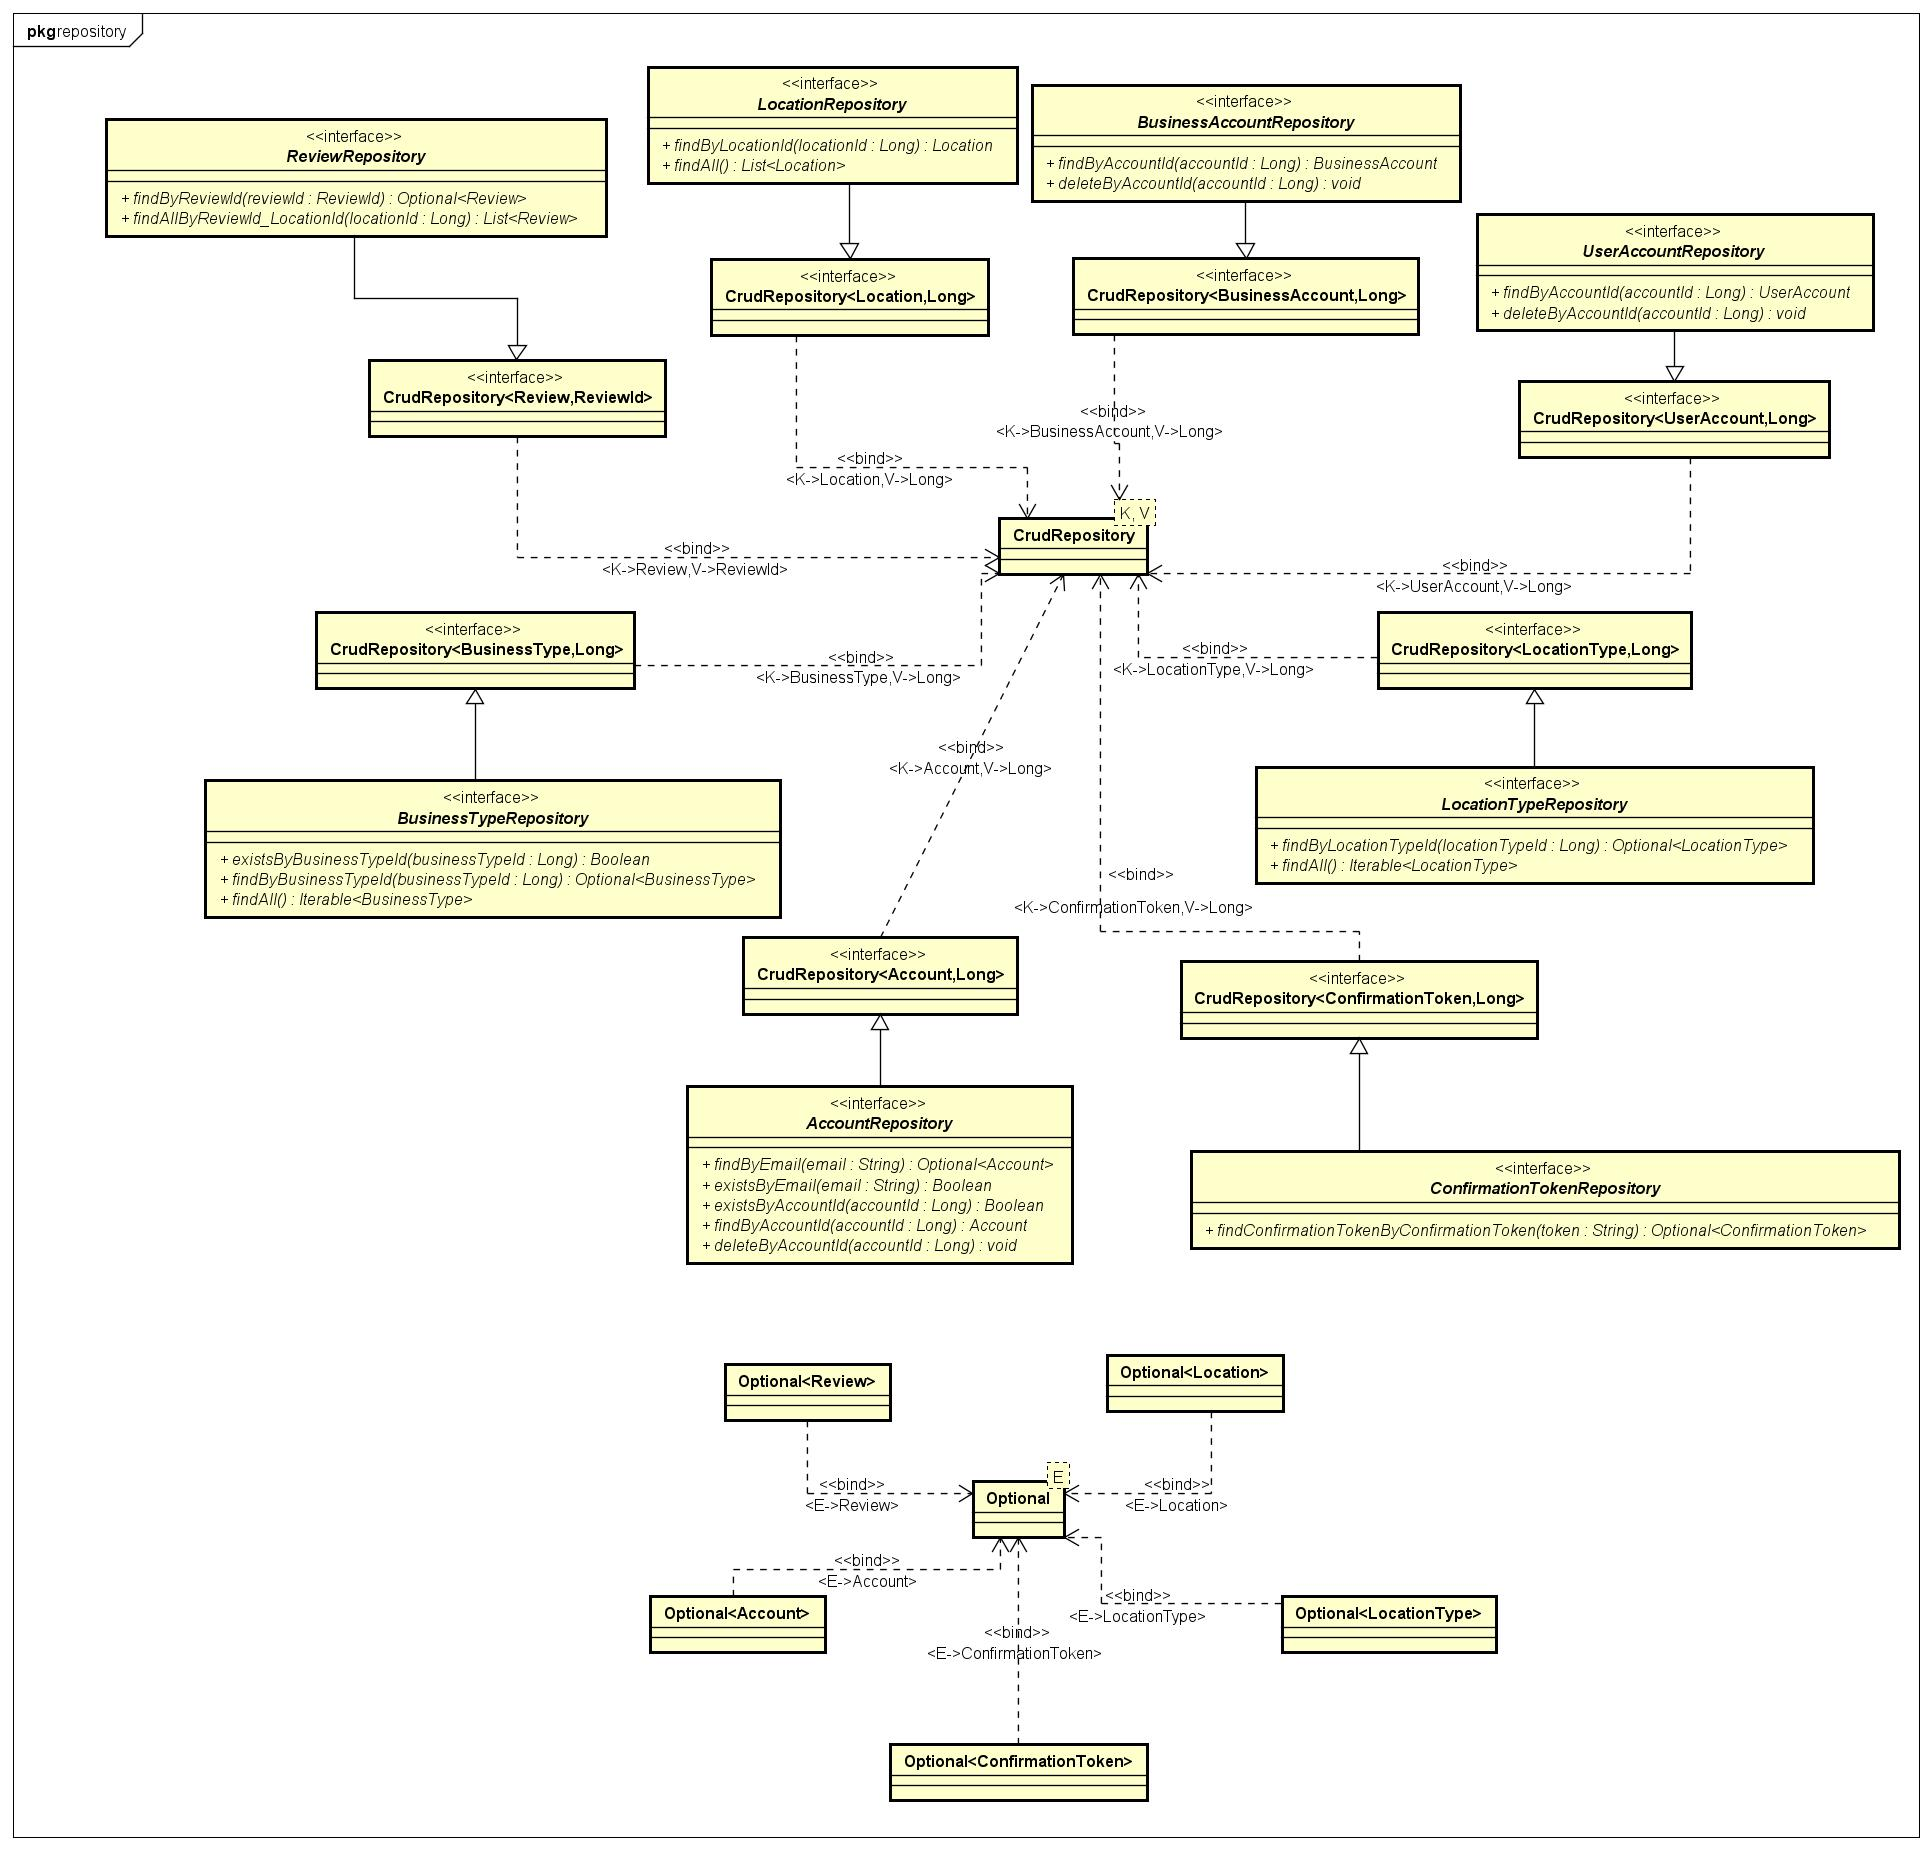
\includegraphics[width=\textwidth]{img/Dijagrami razreda/Repository_Class_Dijagram.jpg}
        	\centering
        	\caption{Repository class}
        	\label{fig:promjene}
        \end{figure}
        \begin{figure}[H]
        	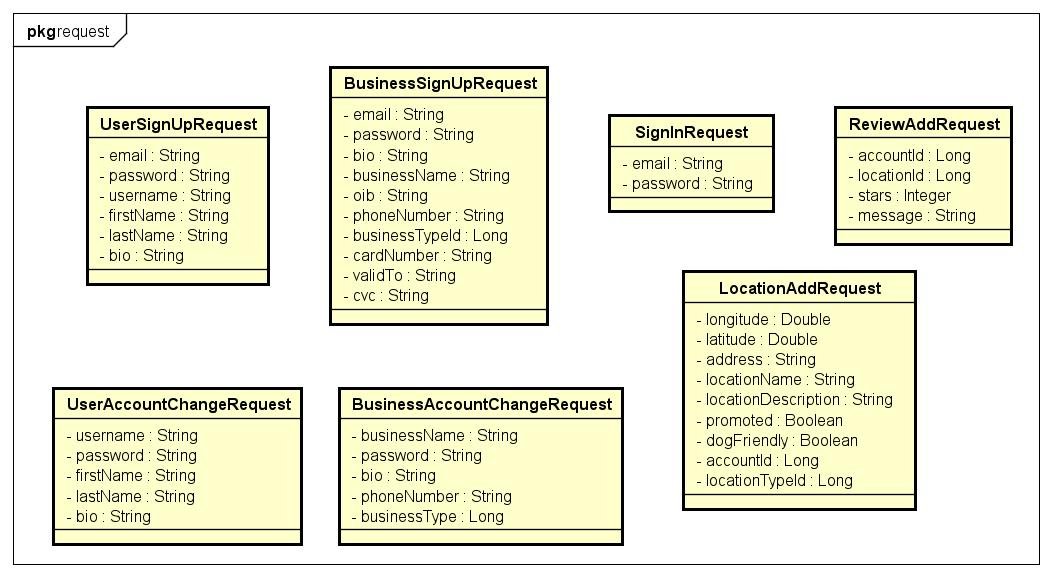
\includegraphics[width=\textwidth]{img/Dijagrami razreda/Request_Class_Dijagram.jpg}
        	\centering
        	\caption{Request class}
        	\label{fig:promjene}
        \end{figure}
        \begin{figure}[H]
        	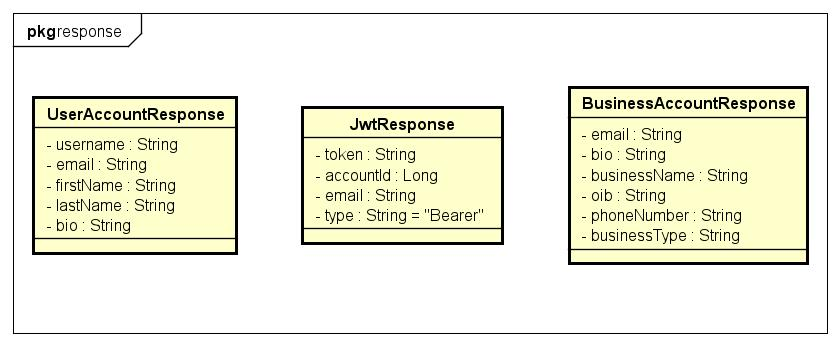
\includegraphics[width=\textwidth]{img/Dijagrami razreda/Response_Class_Dijagram.jpg}
        	\centering
        	\caption{Response class}
        	\label{fig:promjene}
        \end{figure}
        \begin{figure}[H]
        	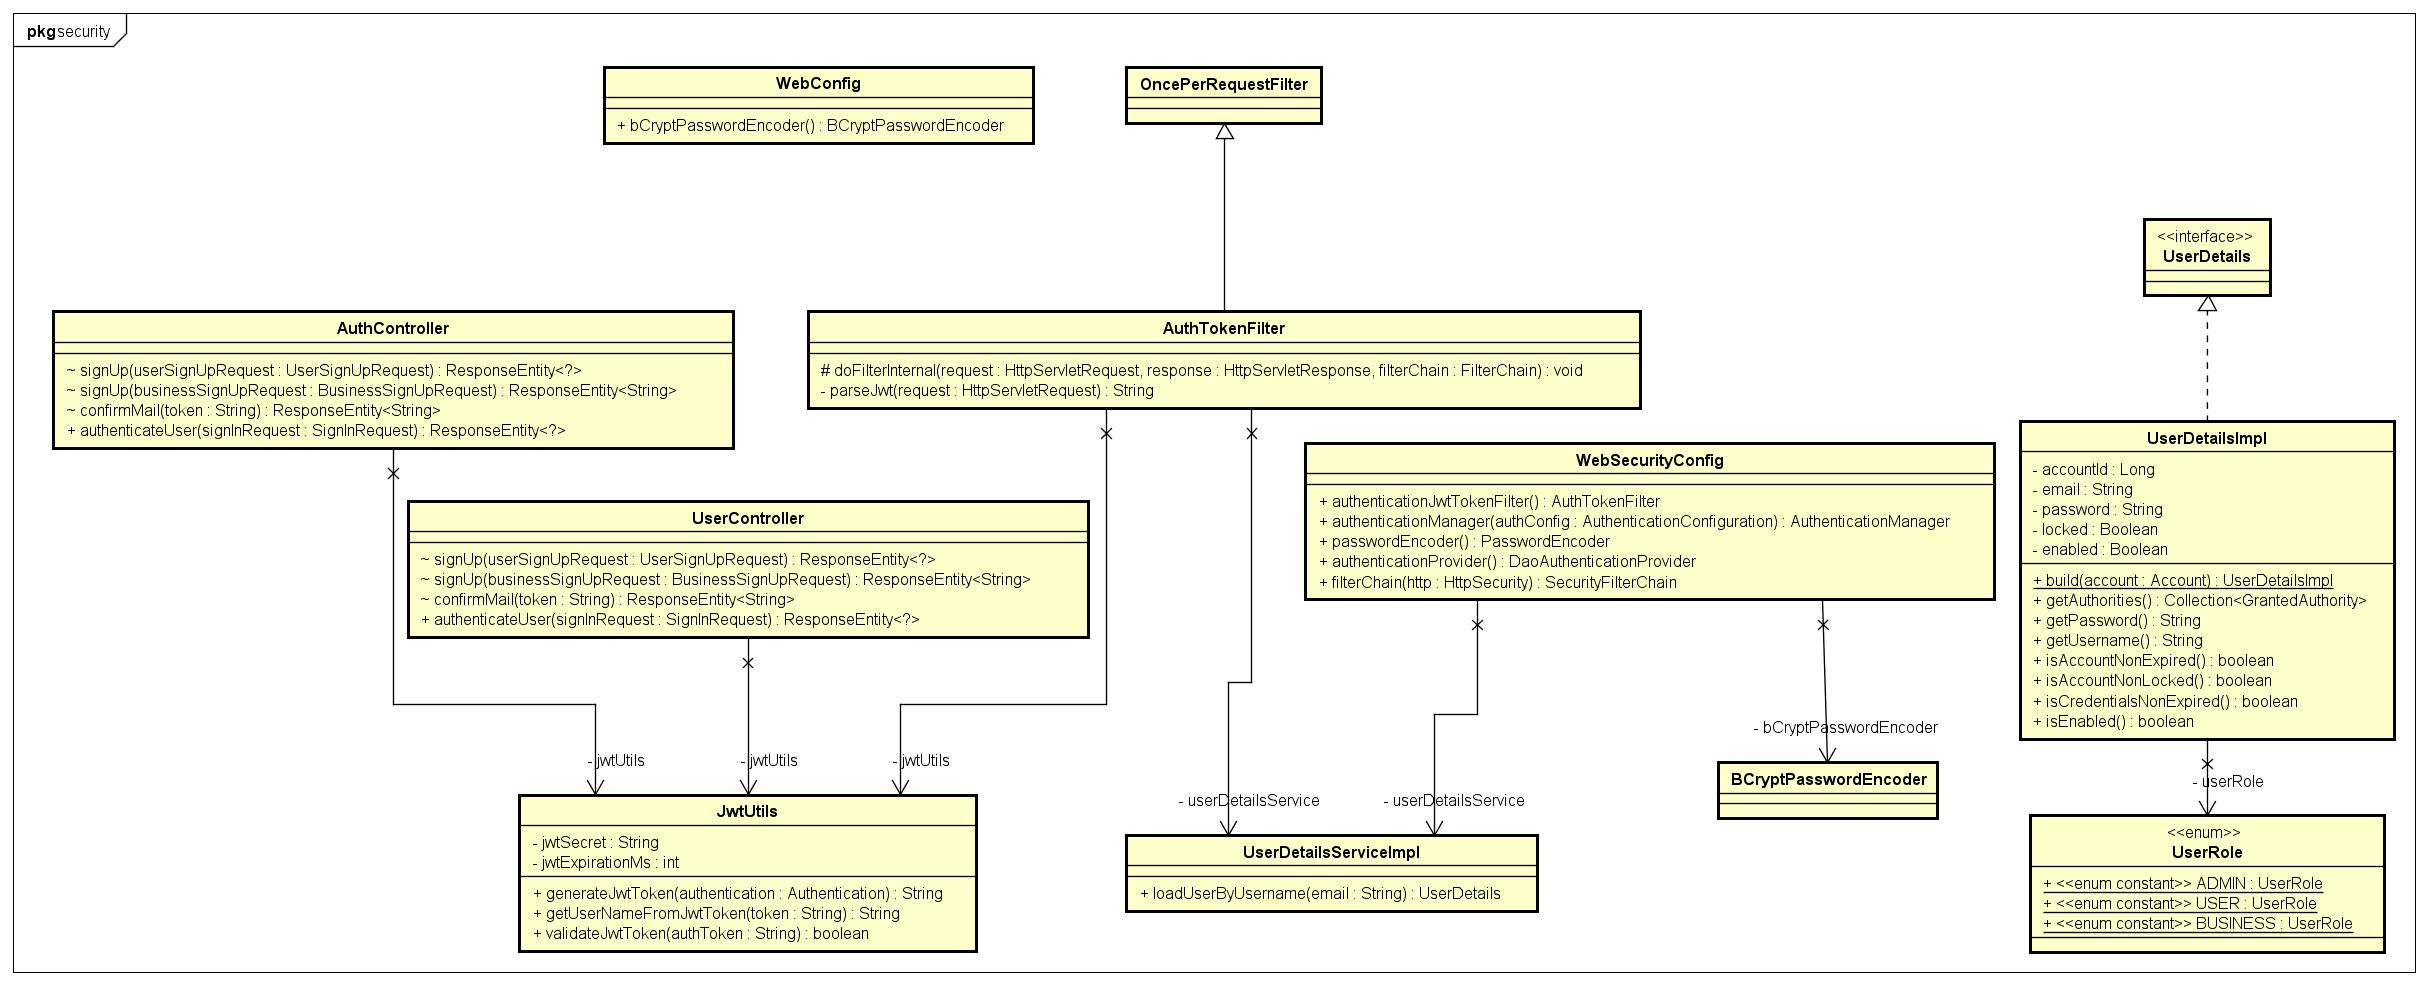
\includegraphics[width=\textwidth]{img/Dijagrami razreda/Security_Class_Dijagram.jpg}
        	\centering
        	\caption{Security class}
        	\label{fig:promjene}
        \end{figure}
        \begin{figure}[H]
        	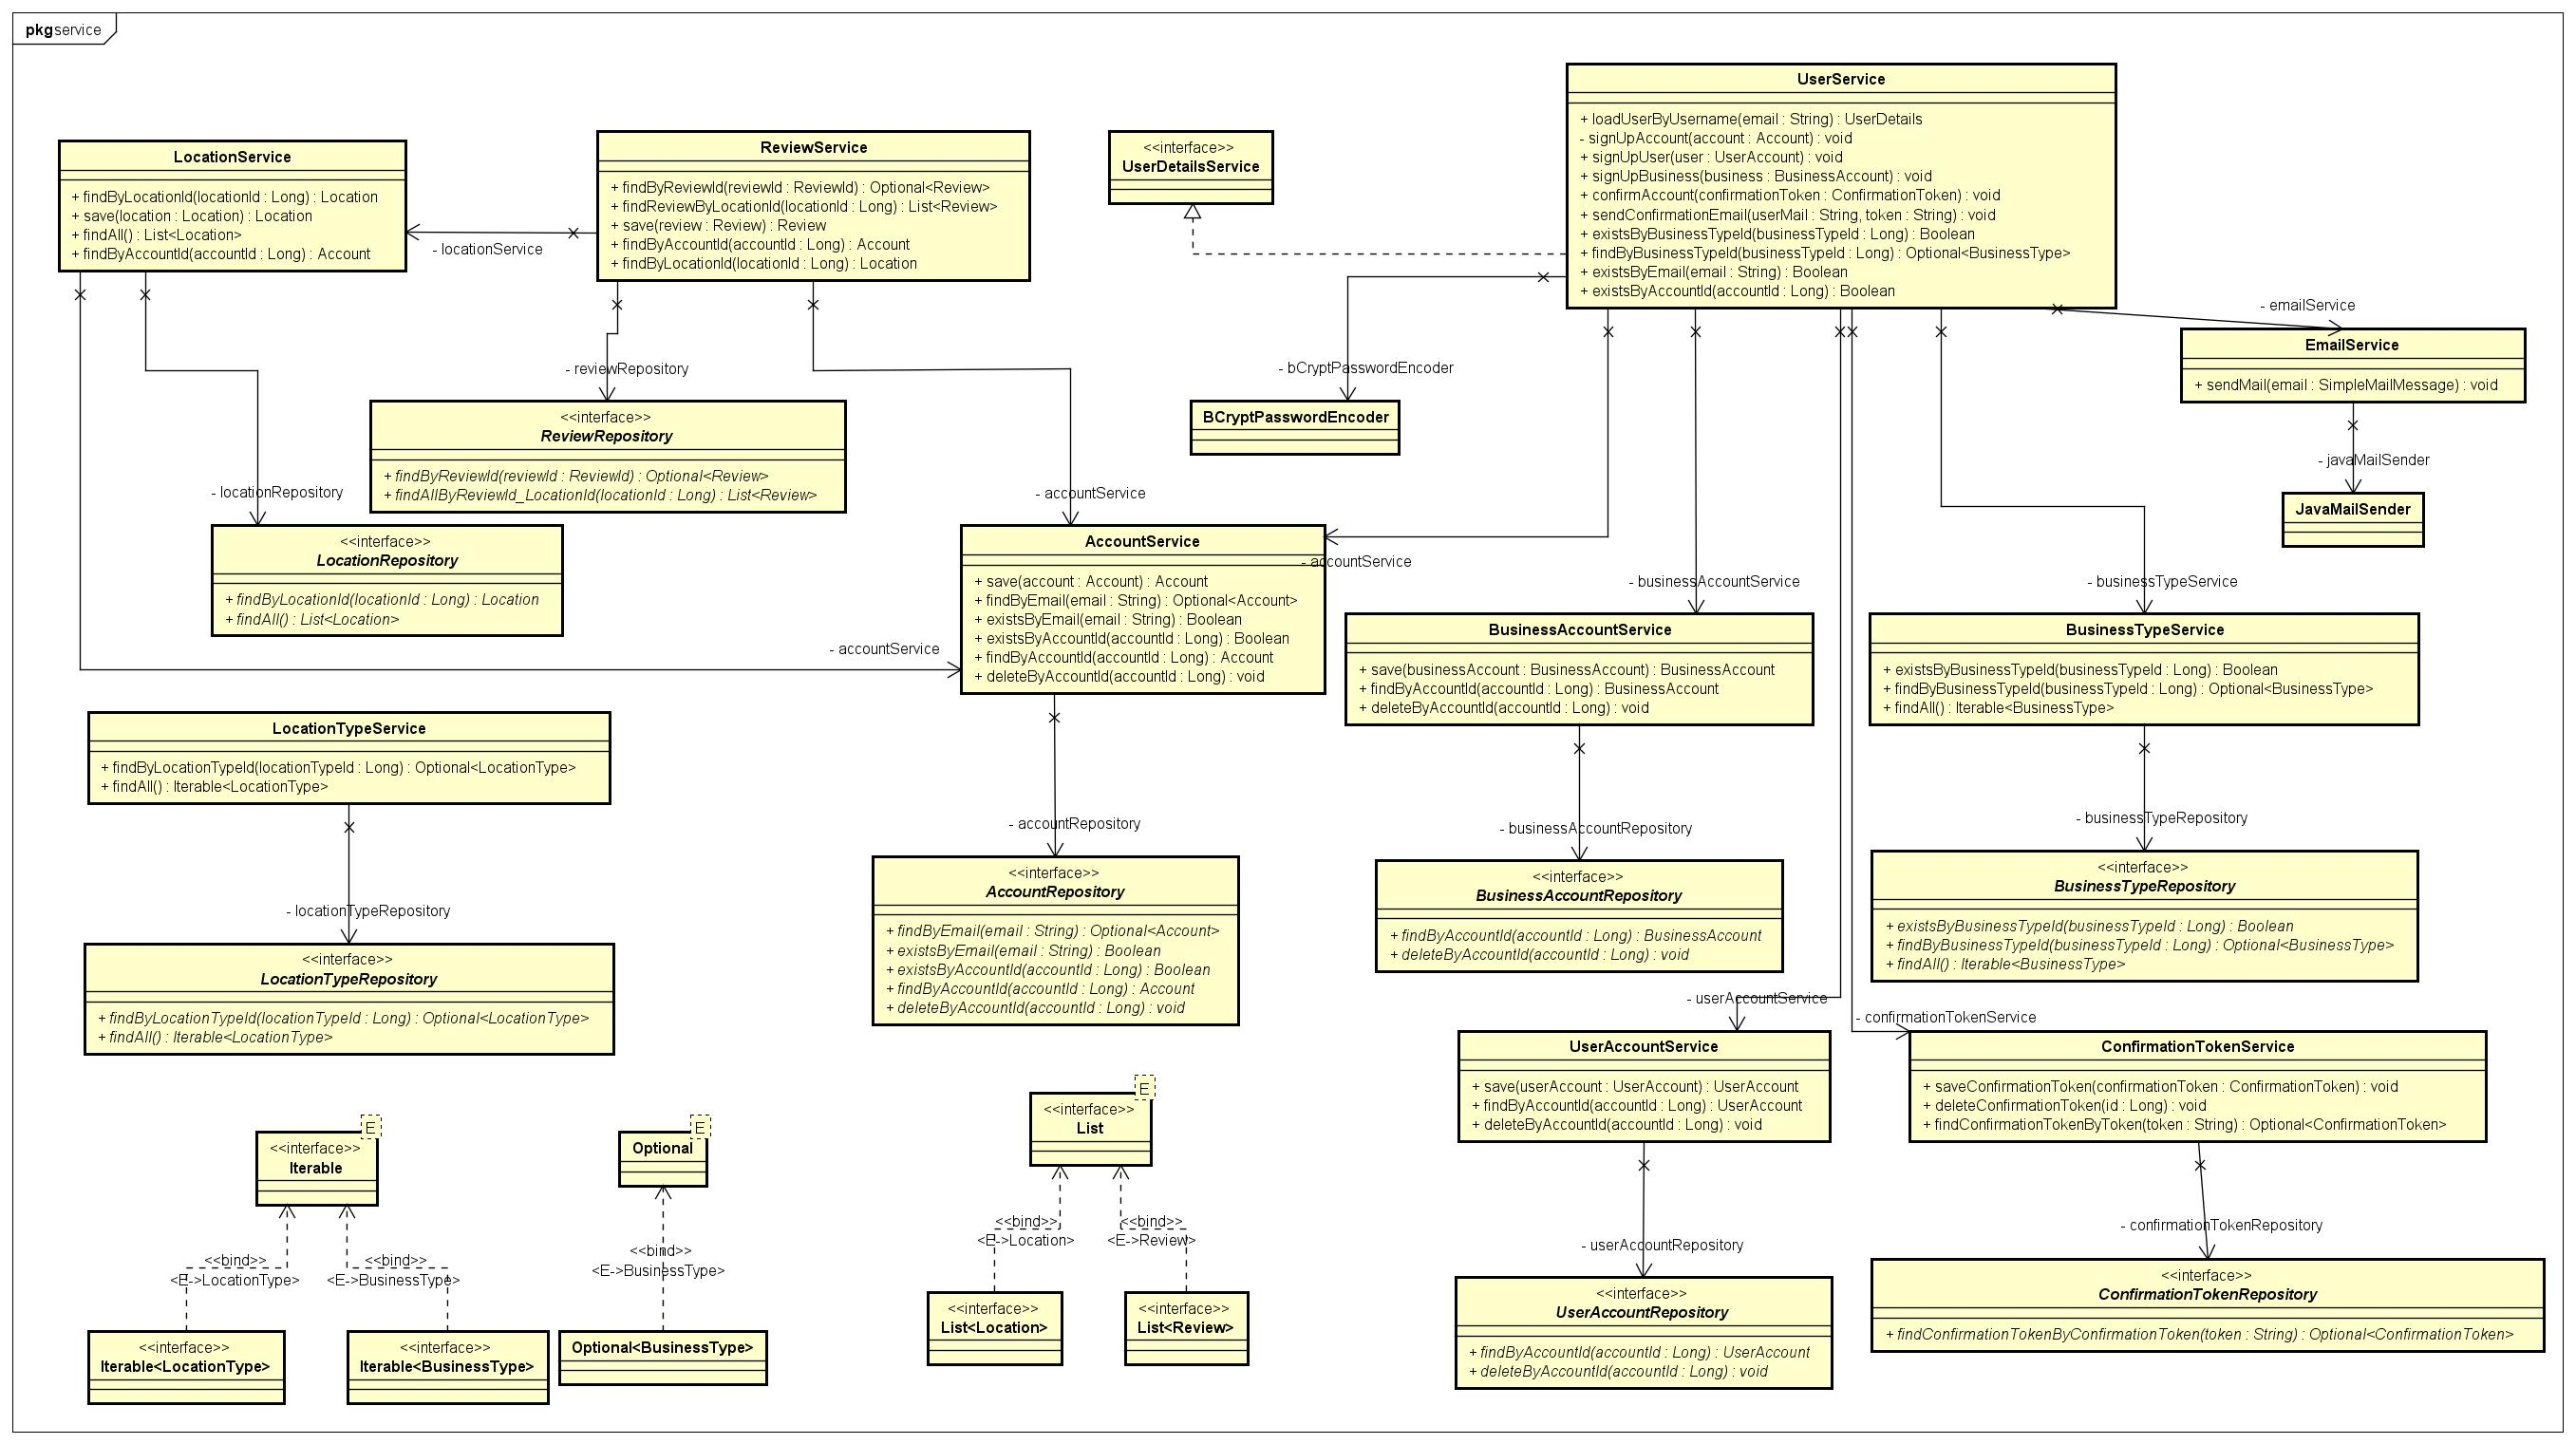
\includegraphics[width=\textwidth]{img/Dijagrami razreda/Service_Class_Dijagram.jpg}
        	\centering
        	\caption{Service class}
        	\label{fig:promjene}
        \end{figure}

        \eject
        \subsection{Dijagram razreda nakon završene aplikacije}
        \begin{figure}[H]
        	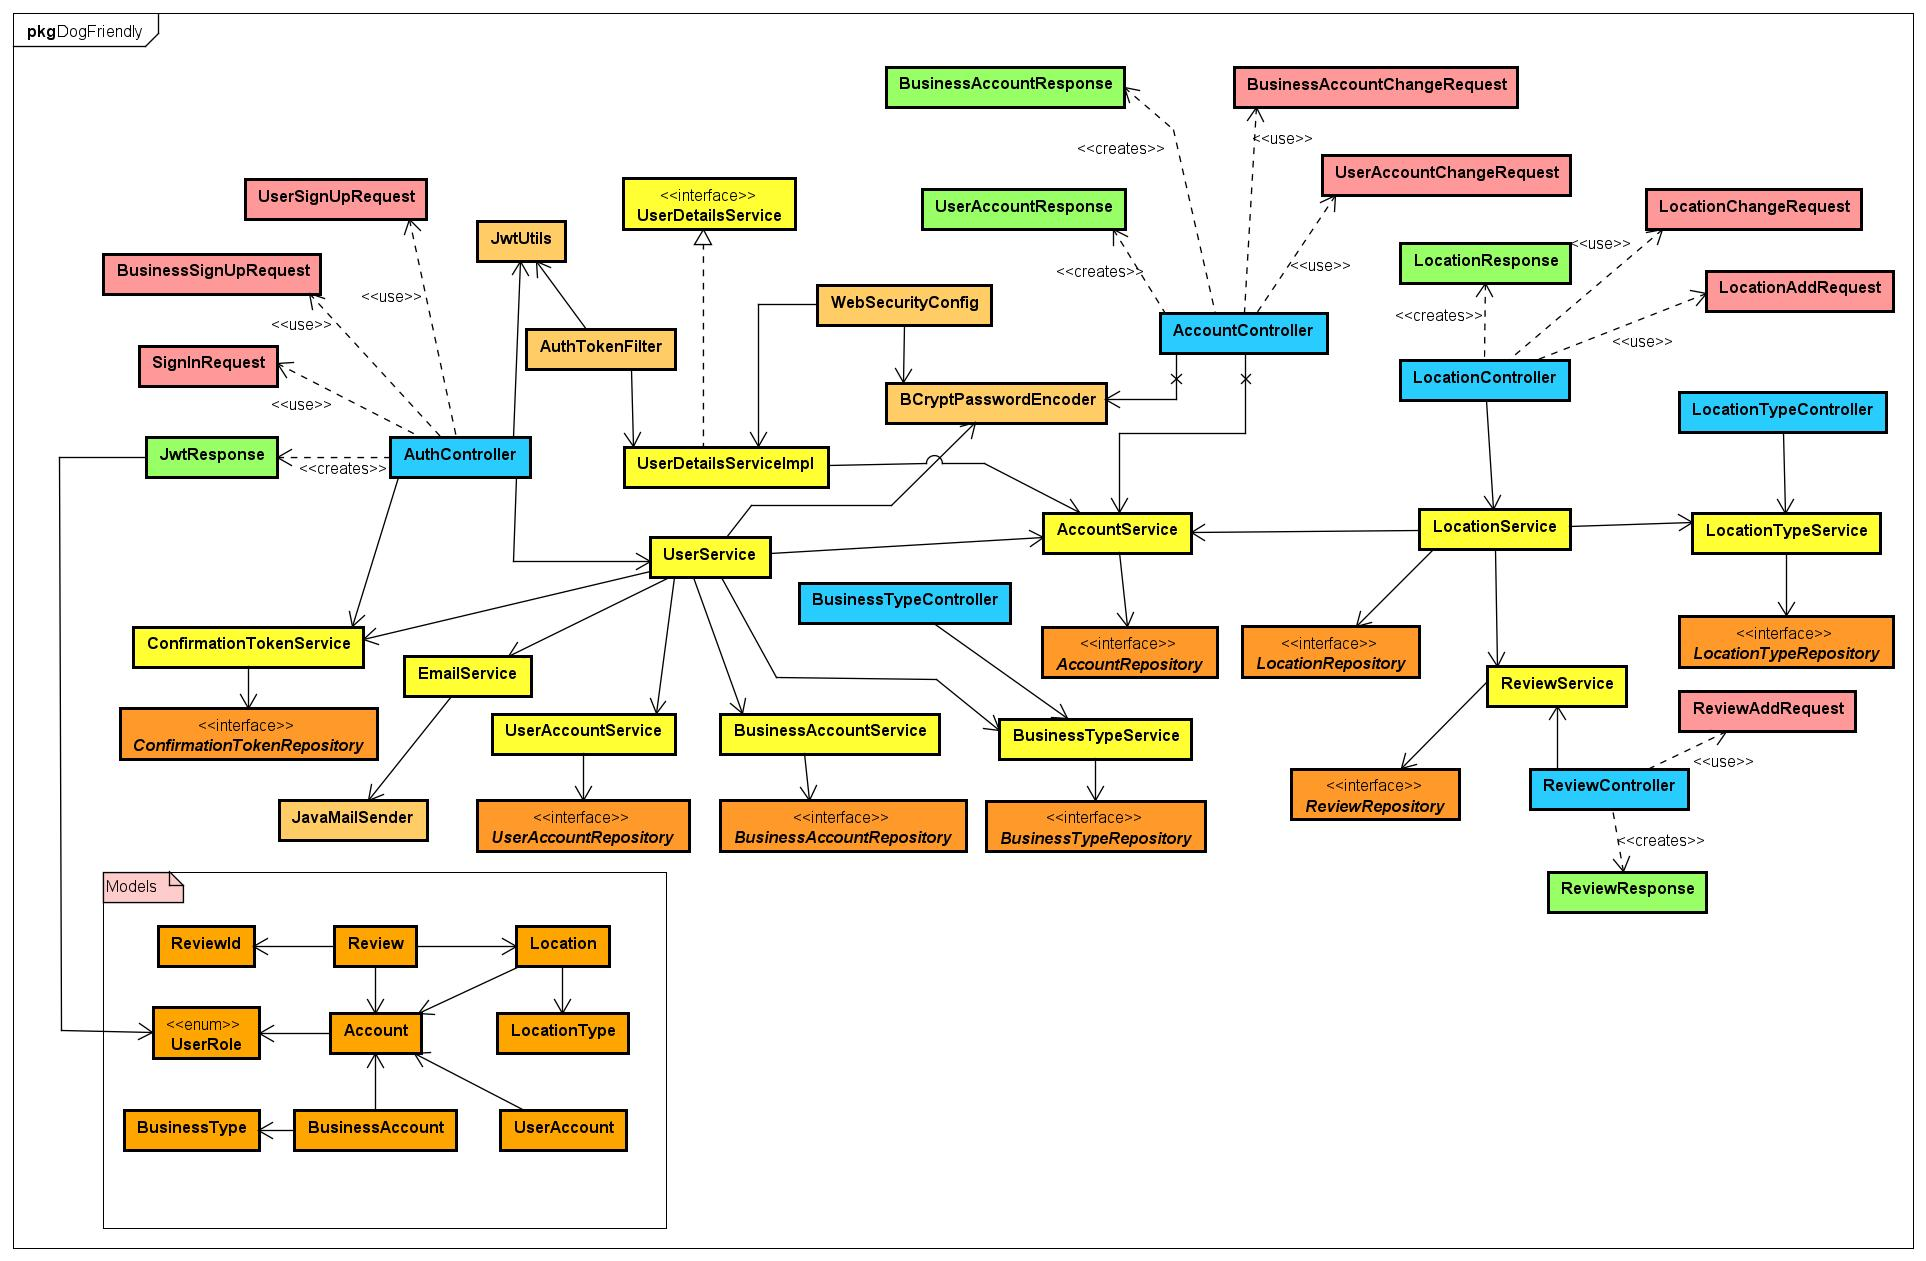
\includegraphics[width=\textwidth]{img/Dijagrami razreda/Class_Diagram.jpg}
        	\centering
        	\caption{Konceptualni dijagram razreda}
        	\label{fig:promjene}
        \end{figure}
    
    \eject
    \section{Dijagram stanja}

        Na slici je prikazan dijagram stanja za prijavljenog korisnika. Korisniku se otvara početna stranica s kartom. U gornjem desnom kutu je gumb koji ga vodi na njegov profil. Na svom profilu korisniku je omogućeno mijenjanje podataka profila ili brisanje računa. Također, sve lokacije koje je korisnik dodao su mu ponuđene na profilu da ih može mijenjati ili obrisati. Do podataka o lokaciji i pisanja recenzije može doći odabirom markera na karti ili pretraživanjem lokacije. Ako pretraživana lokacija ne postoji, korisniku se nudi opcija dodavanja lokacije.

        \begin{figure}[H]
        	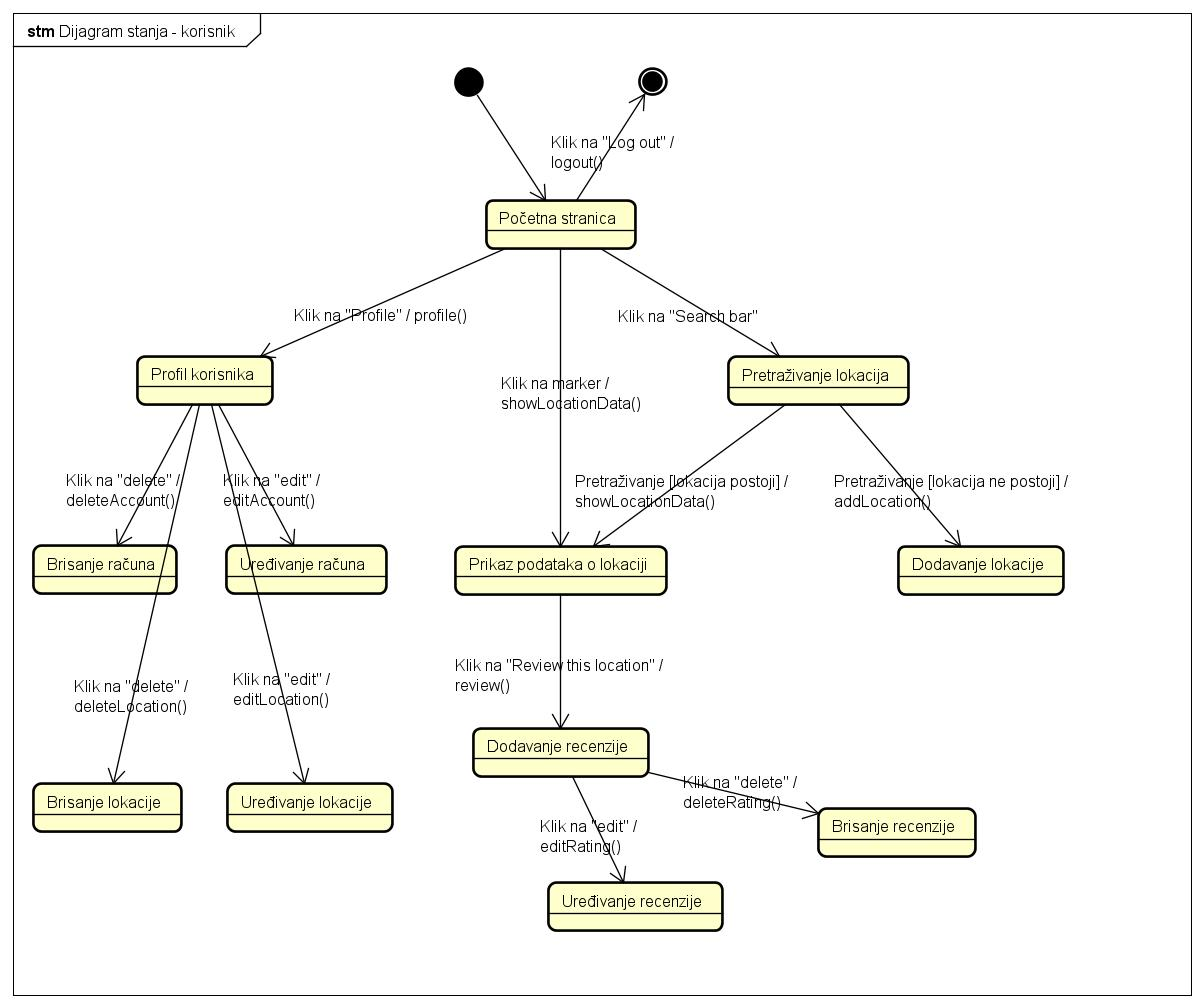
\includegraphics[width=\textwidth]{img/Dijagram stanja - korisnik.jpg}
        	\centering
        	\caption{Dijagram stanja}
        	\label{fig:promjene}
        \end{figure}

        \newpage 
    
    \section{Dijagram aktivnosti}
        Dijagram aktivnosti primjenjuje se za modeliranje upravljačkog i podatkovnog toka. U modeliranju toka upravljanja koristi se “pull” način djelovanja tj. svaki novi korak poduzima se nakon završenog prethodnog. Cilj je jednostavno i sažeto prikazati tok kontrole između pojedinih interakcija. Na dijagramu aktivnosti prikazan je proces pretraživanja i dodavanja lokacija registriranog korisnika. Korisnik, nakon prijave u sustav, pretražuje željenu lokaciju. U slučaju da lokacija već postoji u sustavu, prikazuju mu se podatci o odabranoj lokaciji, u suprotnom, registrirani korisnik ima mogućnost dodati novu vlastitu lokaciju. Ispravnim unosom podataka i ponovnim učitavanjem stranice lokacija postaje vidljiva na karti. 

        \begin{figure}[H]
        	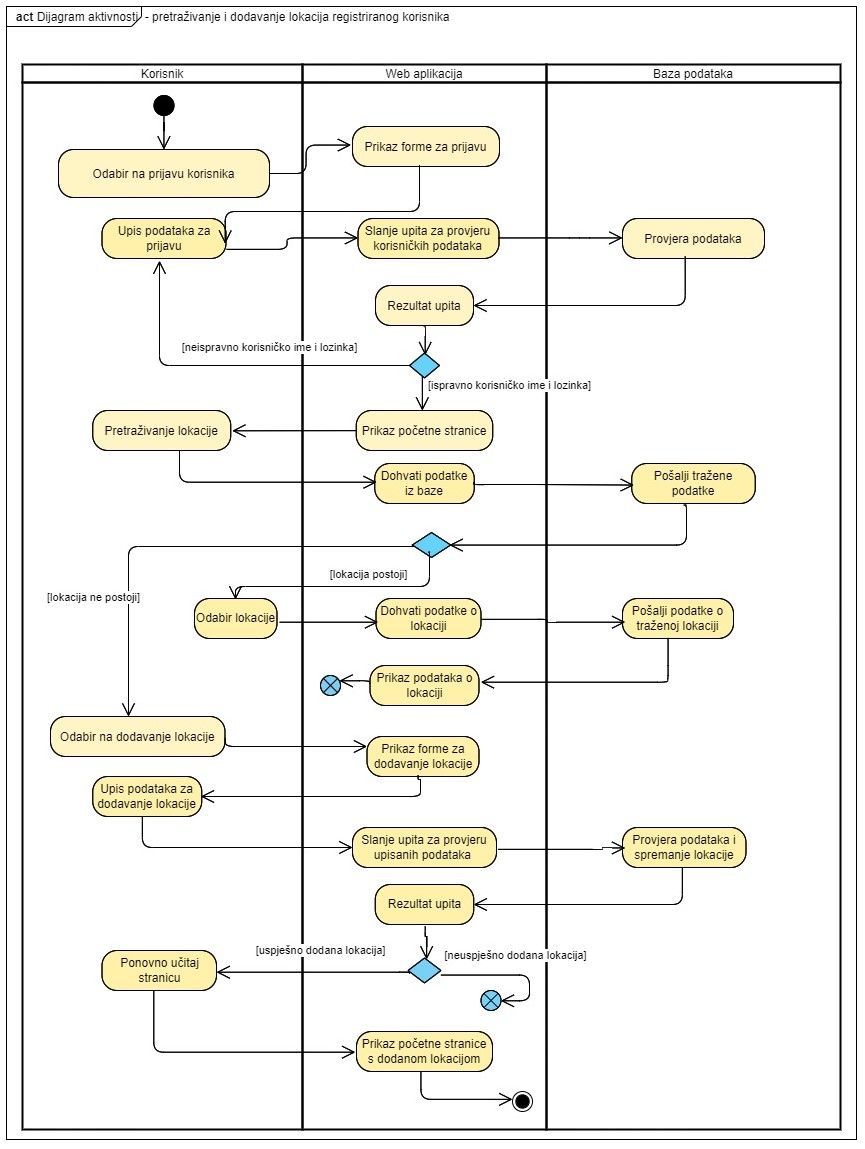
\includegraphics[width=\textwidth]{img/Dijagram aktivnosti.jpg}
        	\centering
        	\caption{Dijagram aktivnosti}
        	\label{fig:promjene}
        \end{figure}
    
    \section{Dijagram komponenti}

        Dijagram komponenti predstavlja specifikaciju arhitekture programske potpore i služi za vizualizaciju međuovisnosti i organizacije između implementacijskih komponenata. Sučeljem za dohvat HTML, CSS i JS datoteka se pristupa nginx komponenti koja poziva index.js. REST API komponenti se pristupa preko sučelja za dohvat JSON datoteka, a ona nam je potrebna za pristup bazi podataka.

        \begin{figure}[H]
        	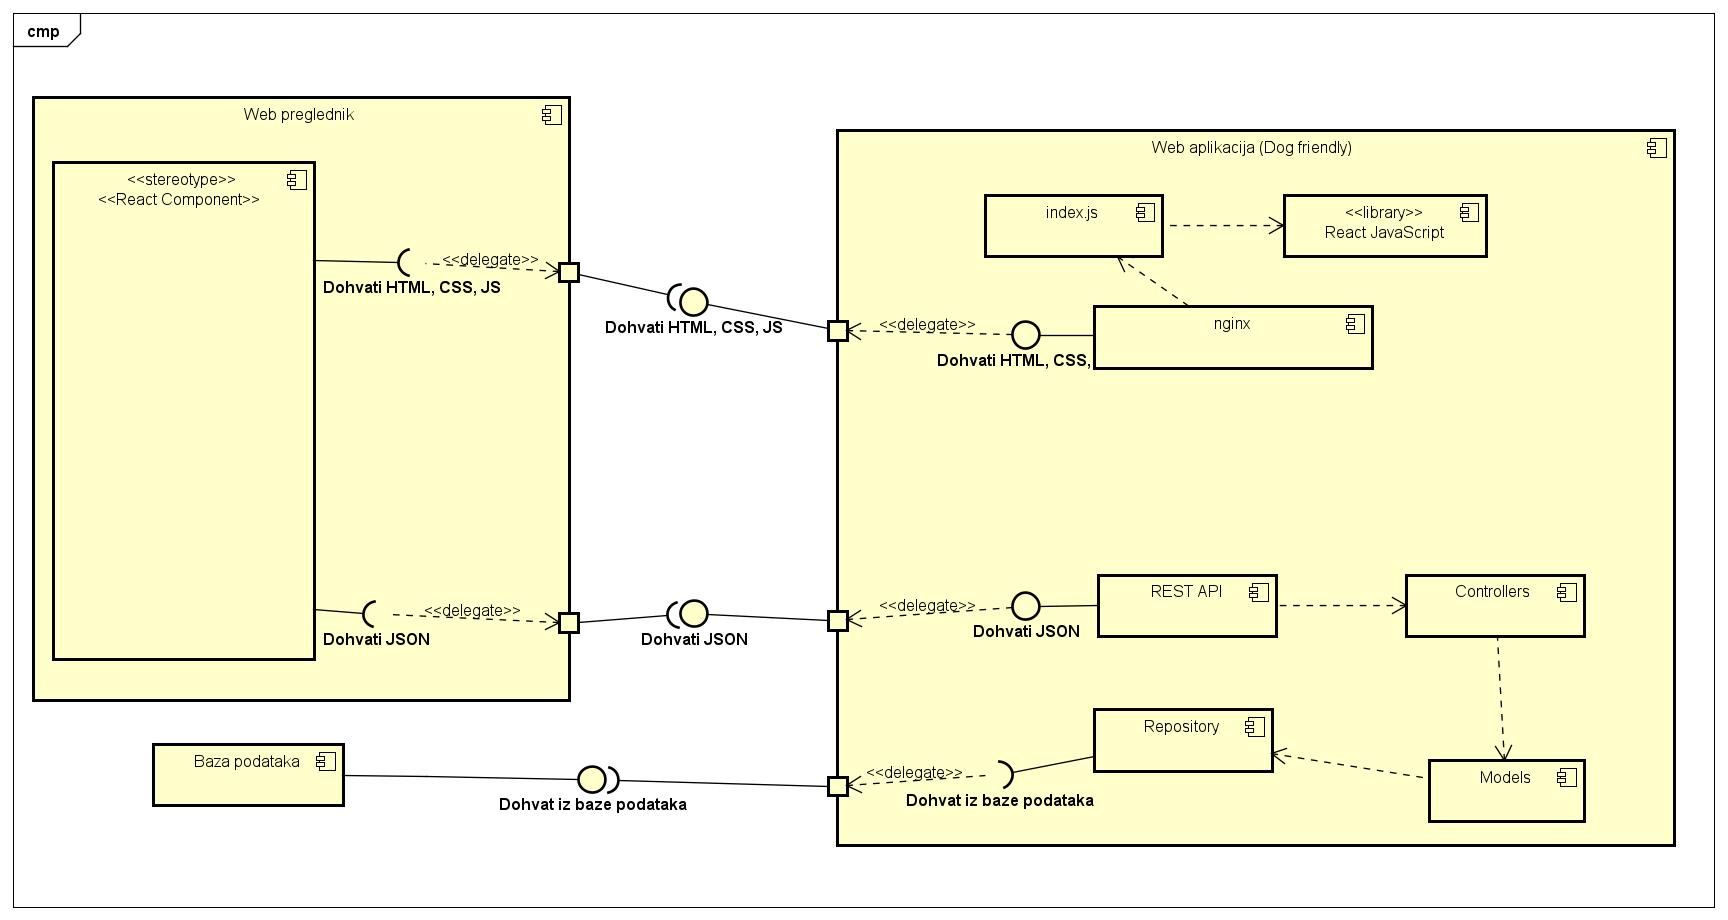
\includegraphics[width=\textwidth]{img/Dijagram komponenti.jpg}
        	\centering
        	\caption{Dijagram komponenti}
        	\label{fig:promjene}
        \end{figure}
    